\begin{problem}{Haruhi with Jenga}{standard input}{standard output}{1 second}

电脑社社长要和 $Haruhi$ 决战叠叠乐大赛!

电研社社长的要求如下:

\begin{itemize}
\item 用电研社自创的叠叠乐游戏一决胜负。
\item 假如我们赢了,目前安置在 $SOS$ 团桌上的电脑,就要乖乖回到原本应在的场所。
\item 归根究底,$SOS$ 团根本就用不到那么好的多功能型电脑,电脑应该是放在电脑研究社才能物尽其用的器材。强烈要求物归原主。
\item 抢夺电脑时带给社长和社员们精神上莫大的苦痛,就趁这机会忘掉吧。不,其实我们也很想忘掉。就彼此都把它忘掉吧。
\item 基于上述的理由,你们必须接受我们的挑战……开战吧!
\end{itemize}

规则如下,一张 $n$ 格长纸条,格子内从左到右依次写着 $1,2,\cdots,n$ 共 $n$ 个数字,每次可以按数字之间的分界线折叠(常规意义下的纸片折叠,与现实完全相同),比如 $1,2,3,4,5$ 折一下变成 $2$ 层,上层 $3,2,1$,下层 $4,5$ 这样的。最后叠来叠去变成 $n$ 层,从上到下形成一个序列。

游戏程式每次会给 $Haruhi$ 一个序列,如果 $Haruhi$ 能折出来就算她赢啦,但是折不出来的话就要满足电研社以上的所有要求。

电研社可能会为了夺回电脑不择手段,所以给出的序列并不一定能够折出来,我们需要帮助 $Haruhi$ 判断这个结果序列是否合法。虽然我还是很希望电研社能赢的,但是为了世界的和平,拜托啦!



\InputFile

第一行一个正整数 $T(1 \leq T \leq 1000)$ ,表示接下来有 $T$ 组数据。

每组的第一行一个正整数 $n(1 \leq n \leq 80)$ 。

每组的第二行有 $n$ 个正整数 $a_1-a_n$ 表示结果序列,数据保证这 $n$ 个数是 $1-n$ 的一个排列。

\OutputFile

对于每组数据输出一行 $yes$ 或 $no$ 表示是否能由原纸片折叠得到。

\Example
\begin{example}
\exmp{
6
5
1 2 3 4 5
5
5 3 1 2 4
4
1 3 2 4
4
2 1 4 3
7
5 2 3 4 1 6 7
7
5 2 3 4 1 7 6
}{
yes
yes
no
yes
yes
yes
}%
\end{example}

\Note
\begin{center}
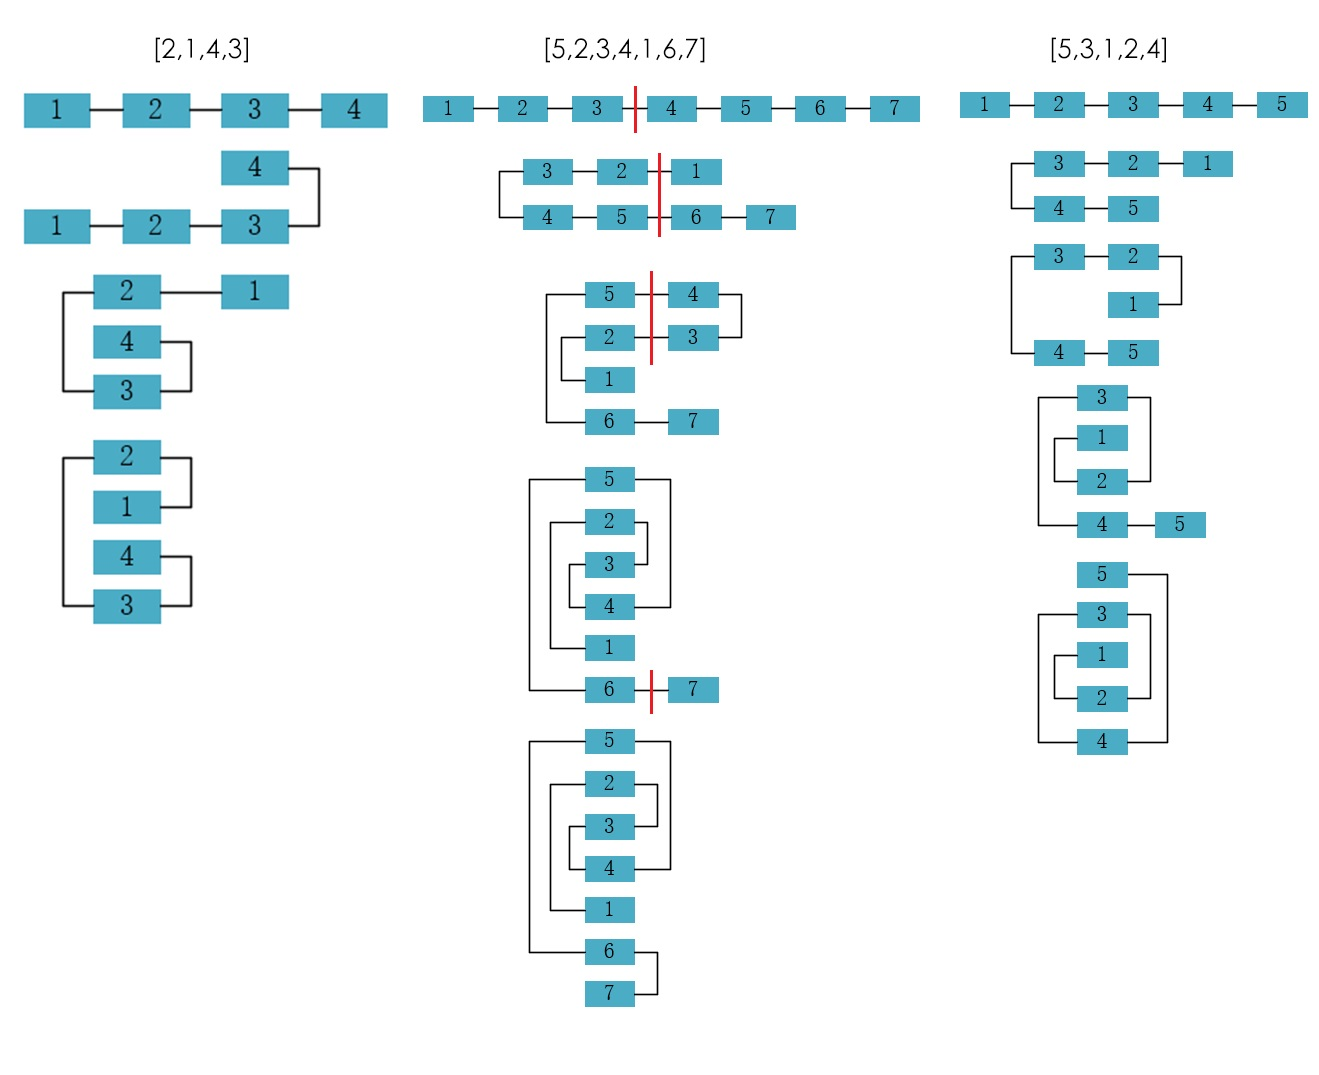
\includegraphics[width=1\textwidth]{pics/J.jpg}
\end{center}

\end{problem}
